% -*- latex -*-
%%%%%%%%%%%%%%%%%%%%%%%%%%%%%%%%%%%%%%%%%%%%%%%%%%%%%%%%%%%%%%%%
%%%%%%%%%%%%%%%%%%%%%%%%%%%%%%%%%%%%%%%%%%%%%%%%%%%%%%%%%%%%%%%%
%%%%
%%%% This text file is part of the source of 
%%%% `Parallel Programming in MPI and OpenMP'
%%%% by Victor Eijkhout, copyright 2012-9
%%%%
%%%% mpi-commsplit.tex : about splitting communicators
%%%%
%%%%%%%%%%%%%%%%%%%%%%%%%%%%%%%%%%%%%%%%%%%%%%%%%%%%%%%%%%%%%%%%
%%%%%%%%%%%%%%%%%%%%%%%%%%%%%%%%%%%%%%%%%%%%%%%%%%%%%%%%%%%%%%%%

\Level 0 {Splitting a communicator}
\label{sec:comm-split}

Splitting a communicator into multiple disjoint communicators
can be done with \indexmpishow{MPI_Comm_split}.
This uses a `colour':
%
\mpiRoutineRef{MPI_Comm_split}
%
and all processes in the old communicator with the same colour
wind up in a new communicator together. The old communicator still exists,
so processes now have two different contexts in which to communicate.

The ranking of processes in the new communicator is determined by a `key' value.
Most of the time, there is no reason to use a relative ranking that is different from
the global ranking, so the \indexmpishow{MPI_Comm_rank} value of the global communicator
is a good choice.

Here is one example of communicator splitting. Suppose your processors
are in a two-dimensional grid:
\begin{lstlisting}
MPI_Comm_rank( MPI_COMM_WORLD, &mytid );
proc_i = mytid % proc_column_length;
proc_j = mytid / proc_column_length;
\end{lstlisting}
You can now create a communicator per column:
\begin{lstlisting}
MPI_Comm column_comm;
MPI_Comm_split( MPI_COMM_WORLD, proc_j, mytid, &column_comm );
\end{lstlisting}
and do a broadcast in that column:
\begin{lstlisting}
MPI_Bcast( data, /* tag: */ 0, column_comm );
\end{lstlisting}
Because of the SPMD nature of the program, you are now doing in parallel
a broadcast in every processor column. Such operations often appear
in \indexterm{dense linear algebra}.

The \indexmpishow{MPI_Comm_split} routine has a `\n{key}' parameter,
which controls how the processes in the new communicator are
ordered. By supplying the rank from the original communicator you let
them be arranged in the same order.

\begin{figure}[ht]
  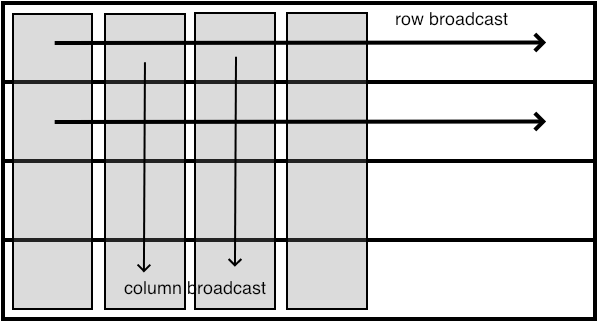
\includegraphics[scale=.1]{procgrid-bcast}
  \caption{Row and column broadcasts in subcommunicators}
  \label{fig:procgrid-bcast}
\end{figure}

One application of communicator splitting is setting up a processor
grid, with the possibility of using MPI solely within one row or
column; see figure~\ref{fig:procgrid-bcast}.

\begin{exercise}
  \label{ex:rowcolcomm}
  Organize your processes in a grid, and make subcommunicators for
  the rows and columns. For this compute the row and column number of
  each process.

  In the row and column communicator, compute the rank. For instance,
  on a $2\times3$ processor grid you should find:
\begin{verbatim}
Global ranks:  Ranks in row:  Ranks in colum:
  0  1  2      0  1  2        0  0  0
  3  4  5      0  1  2        1  1  1
\end{verbatim}

  Check that the rank in the row communicator is the column number,
  and the other way around.

  Run your code on different number of processes, for instance a
  number of rows and columns that is a power of~2, or that is a prime number.
\begin{tacc}
    This is one occasion where you could use \n{ibrun -np 9};
    normally you would \emph{never} put a processor count on \n{ibrun}.
\end{tacc}
\end{exercise}

As an example of communicator splitting, consider the recursive
algorithm for \indextermbus{matrix}{transposition}.
Processors are organized in a square grid. The matrix is divided
on $2\times 2$ block form.

\begin{exercise}
  \label{ex:recursivetranspose}
  Implement a recursive algorithm for matrix transposition:
  
  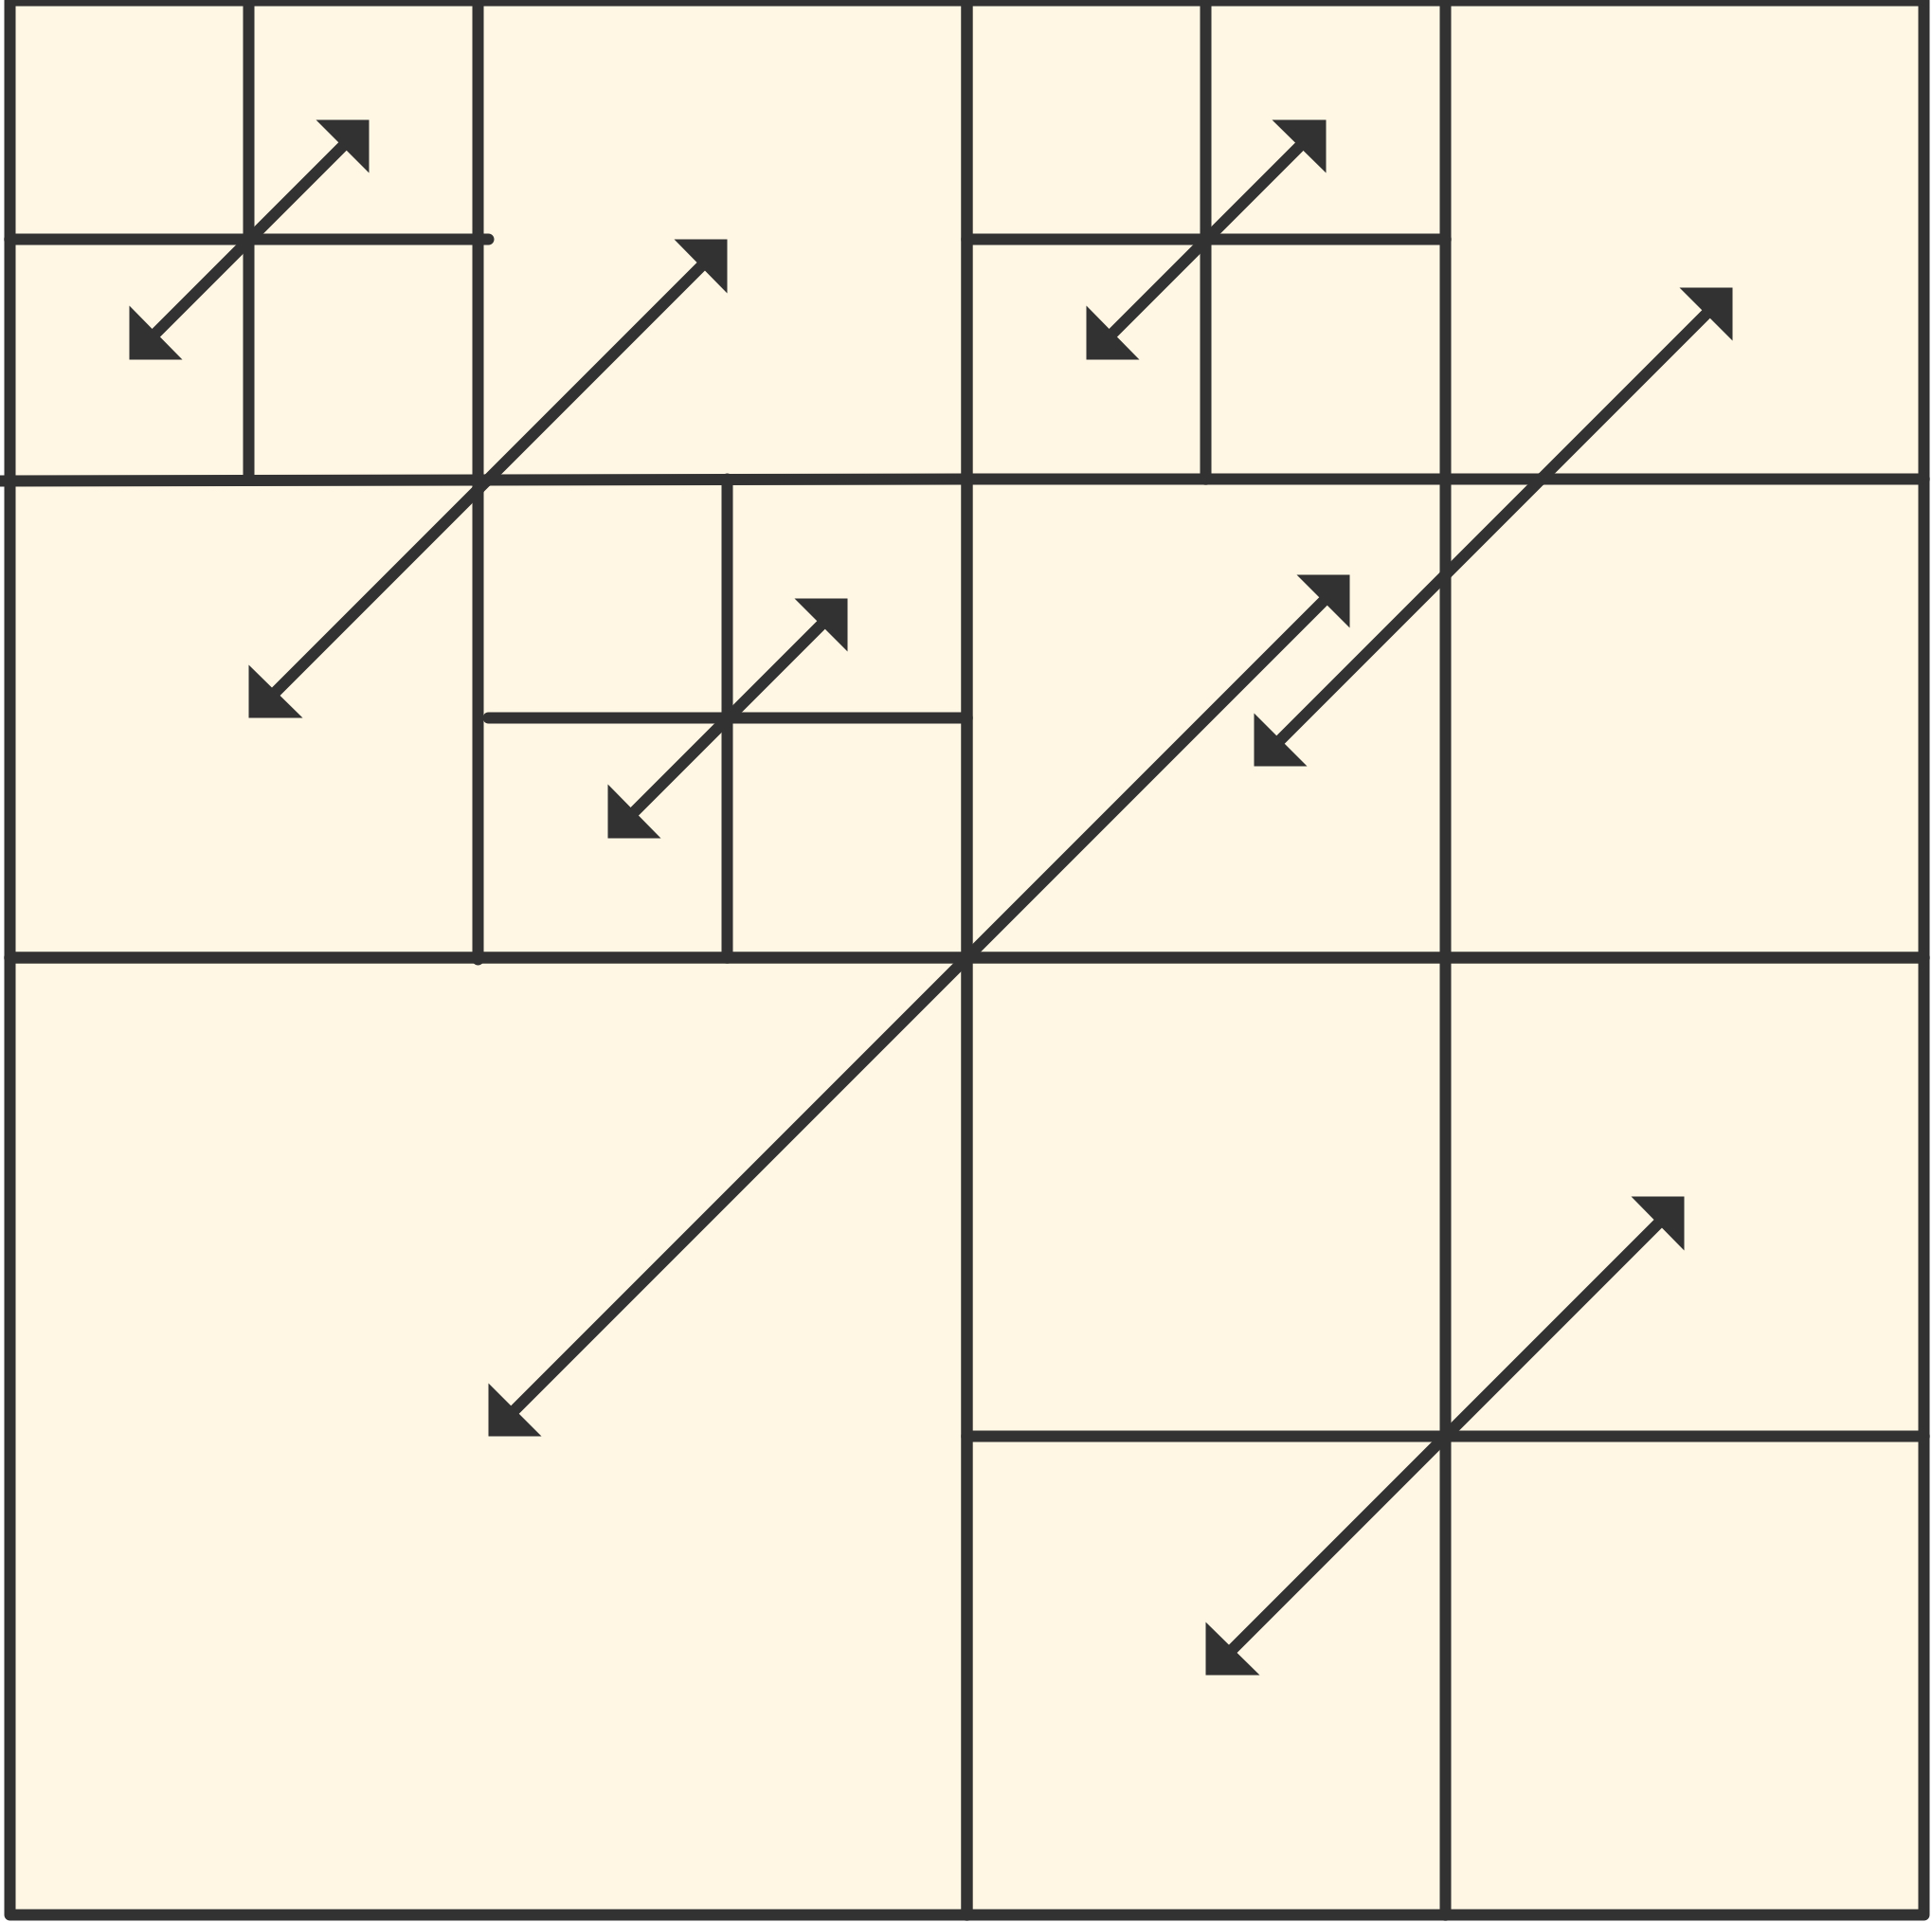
\includegraphics[scale=.1]{recursive-transpose}

  \begin{itemize}
  \item Swap blocks $(1,2)$ and $(2,1)$; then
  \item Divide the processors into four subcommunicators, and
    apply this algorithm recursively on each;
  \item If the communicator has only one process, transpose the matrix in place.
  \end{itemize}
\end{exercise}

There is an important application of communicator splitting in the
context of one-sided communication, grouping processes by whether they
access the same shared memory area; see section~\ref{mpi-comm-split-type}.

\Level 1 {Process groups}

The most general mechanism is based on groups: you can extract the
group from a communicator, combine different groups, and form a new
communicator from the resulting group.

The group mechanism is more involved. You get the group from a
communicator with \indexmpishow{MPI_Comm_group},
or conversely make a communicator from a group with \indexmpishow{MPI_Comm_create}.

\mpiRoutineRef{MPI_Comm_create}

Creating a new communicator from a group is collective on the old communicator.
There is also a routine \indexmpishow{MPI_Comm_create_group} that only
needs to be called on the group that constitutes the new communicator.

Groups are manipulated with
\indexmpishow{MPI_Group_incl}, \indexmpishow{MPI_Group_excl},
\indexmpishow{MPI_Group_difference} and a few more.

You can name your communicators with \indexmpishow{MPI_Comm_set_name}, which
could improve the quality of error messages when they arise.

\begin{lstlisting}
MPI_Comm_group (comm, group, ierr)
MPI_Comm_create (MPI_Comm comm,MPI_Group group, MPI_Comm newcomm, ierr)
\end{lstlisting}

\begin{lstlisting}
MPI_Group_union(group1, group2, newgroup, ierr)
MPI_Group_intersection(group1, group2, newgroup, ierr)
MPI_Group_difference(group1, group2, newgroup, ierr)
\end{lstlisting}

\begin{lstlisting}
MPI_Group_incl(group, n, ranks, newgroup, ierr)
MPI_Group_excl(group, n, ranks, newgroup, ierr)
\end{lstlisting}
\begin{lstlisting}
MPI_Group_size(group, size, ierr)
MPI_Group_rank(group, rank, ierr)
\end{lstlisting}

\Level 1 {Intra-communicators}
\label{sec:comm-group}

We start by exploring the mechanisms for creating a communicator that
encompasses a subset of \indexmpishow{MPI_COMM_WORLD}. 

The most general mechanism for creating communicators is through
process groups: you can query the group of processes of a
communicator, manipulate groups, and make a new communicator out of a
group you have formed.

